\section{一个有趣的应用:可撤销的广播加密}

电影公司花费大量精力制作大片,然后将电影(DVD)卖给数以百万计的客户,这些客户购买电影后就可以在家里观看它们。客户应该能够在一个没有网络连接的,无状态的独立电影播放器上观看电影。

然而,电影公司担心盗版问题,并不想把受版权保护的数字内容简单直接地以明文发送给数以百万计的用户。一个简单的解决方案是这样运行的。每个授权制造商都有一个\textbf{设备密钥} $k_\mathrm{d}\in\mathcal{K}$,它会把这个密钥嵌入到它所销售的每台设备中。如果有一百个授权设备制造商,那么就有一百个设备密钥 $k^{(1)}_\mathrm{d}, \dots, k^{(100)}_\mathrm{d}$。一部电影 $m$ 会被加密为:
\[
c_\mathrm{m}:=
\left\{
\begin{aligned}
& k\overset{\rm R}\leftarrow\mathcal{K}\\
& \text{for } i=1,\dots,100\;:\; c_i\leftarrow E(k^{(i)}_\mathrm{d},\,k)\\
& c\overset{\rm R}\leftarrow E'(k,m)\\
& \text{output } (c_1,\dots,c_{100},\;c)
\end{aligned}
\right\}
\]
其中 $(E,D)$ 是一个 CPA 安全的密码,并且在密钥空间为 $\mathcal{K}$ 的情况下,$(E',D')$ 是语义安全的。我们在练习 5.4 中分析了这个构造,我们在该练习中表明,这个构造是 CPA 安全的。我们将 $(c_1, \dots, c_{100})$ 称为密文头部,将 $c$ 称为密文体。

现在,每个授权设备都可以使用内嵌的设备密钥来解密电影。首先解密密文头部中适当的密文,然后使用获得的密钥 $k$ 来解密密文体。这种机制构成了用于加密 DVD 的\textbf{内容加扰系统(content scrambling system, CSS)}的基础。我们之前在 \ref{sec:3-8} 节中曾经遇到过 CSS。

这个方案的麻烦之处在于,一旦某一个设备被攻破,并且它的设备密钥 $k_\mathrm{d}$ 被提取并公布,那么任何人都可以用这个 $k_\mathrm{d}$ 来解密所有曾经发布过的电影。如果不破坏与之关联的许多消费者设备,就没有办法撤销 $k_\mathrm{d}$。事实上,这正是 CSS 被破解的方式:从某一台被授权的播放器中提取出设备密钥,然后使用一个名为 \textbf{DeCSS} 的系统解密被加密的 DVD。

从 CSS 中得到的教训是,全局不可撤销的设备密钥是一个很坏的主意。一旦单个密钥被泄露,所有的安全性都会丧失。当电影行业的硬件载体从 DVD 升级到蓝光时,它们获得了一次重新设计加密方案的机会。在这个被称为\textbf{高级访问内容系统 (Advanced Access Content System, AACS)} 的新方案中,每台设备都包含一个随机的设备密钥,且它对该设备是独一无二的。该系统的设计目标是支持数十亿台设备,并且让每台设备都有自己的密钥。

该系统的目标包含两个方面。首先,每个被授权的设备都应该能够解密每张蓝光光盘。第二,每当一个设备的密钥被提取和公布时,它应当可以被撤销,这使得这个设备的密钥不能被用来解密之后的蓝光光盘,但不会影响到任何其他的设备。

\begin{snote}[一个可撤销的广播系统。]
假设系统中有 $n$ 台设备,为了简单起见,我们假设 $n$ 是 $2$ 的整数次幂。我们把这 $n$ 台设备当作一个完全二叉树的叶子结点,如图 \ref{fig:5-5} 所示。二叉树上的每个结点都被分配了一个密钥空间 $\mathcal{K}$ 中的随机密钥。编号为 $i\in\{1,\dots,n\}$ 的设备中嵌入的密钥就是从编号为 $i$ 的叶子结点到根结点路径上所有密钥的集合。这样,每个设备都恰好被赋予了 $\log_2n$ 个 $\mathcal{K}$ 中的密钥。

当系统第一次启动时,还没有设备的密钥被撤销,所有的内容都是用根结点的密钥(图 \ref{fig:5-5} 中的编号为 $15$ 的密钥)加密的。更确切地说,一部电影 $m$ 会被加密为:
\[
c_\mathrm{m}:=
\left\{
\;
k\overset{\rm R}\leftarrow\mathcal{K},\;
c_1\overset{\rm R}\leftarrow E(k_\mathrm{root},\,k),\;
c\overset{\rm R}\leftarrow E'(k,m),\;
\text{output } (c_1,c)\;
\right\}
\]
因为所有设备都有根密钥 $k_\mathrm{root}$,所有设备都可以解密。
\end{snote}

%\begin{figure}
%  \centering
%  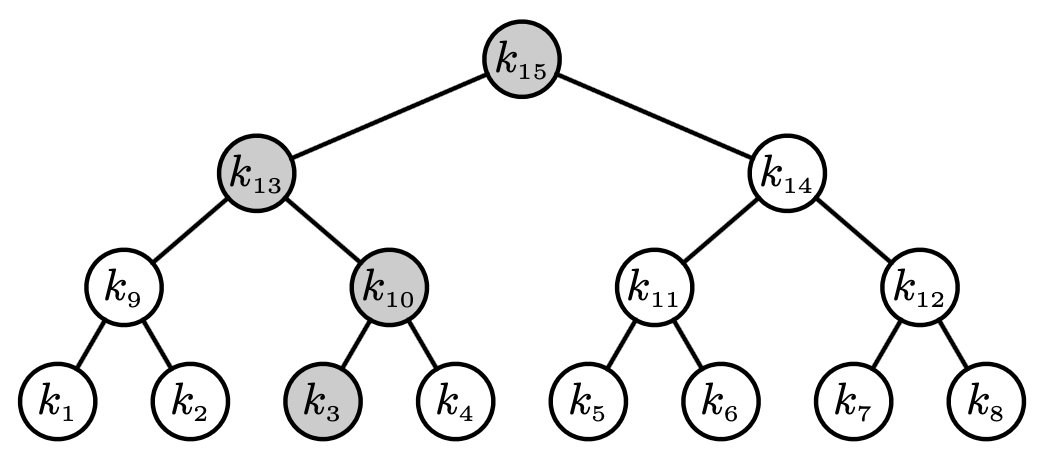
\includegraphics[width=0.45\linewidth]{figures/chapter5/fig5.png}
%  \caption{$n=8$个设备时的密钥树;被阴影标记的结点是嵌入设备 $3$ 中的密钥。}
%  \label{fig:5-5}
%\end{figure}

\begin{figure}
  \centering
  

\tikzset{every picture/.style={line width=0.75pt}} %set default line width to 0.75pt        

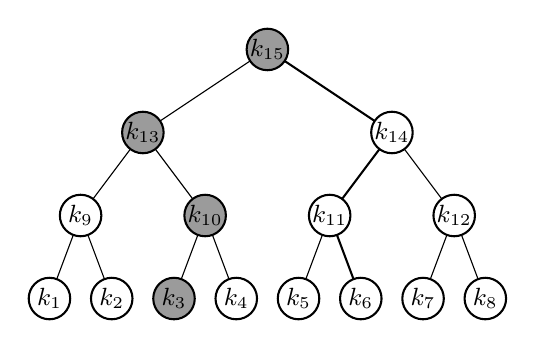
\begin{tikzpicture}[x=0.75pt,y=0.75pt,yscale=-1,xscale=1]
%uncomment if require: \path (0,156); %set diagram left start at 0, and has height of 156

%Straight Lines [id:da07527174742353382] 
\draw    (25,90) -- (10,130) ;
%Straight Lines [id:da35665594344693563] 
\draw    (25,90) -- (40,130) ;
%Straight Lines [id:da7198526785953758] 
\draw    (85,90) -- (70,130) ;
%Straight Lines [id:da8225492469926641] 
\draw    (85,90) -- (100,130) ;
%Straight Lines [id:da9323962351398181] 
\draw    (145,90) -- (130,130) ;
%Straight Lines [id:da9312802340344666] 
\draw [line width=0.75]    (145,90) -- (160,130) ;
%Straight Lines [id:da6015414712737466] 
\draw    (205,90) -- (190,130) ;
%Straight Lines [id:da843374207822494] 
\draw    (205,90) -- (220,130) ;
%Straight Lines [id:da5705947708549455] 
\draw    (55,50) -- (25,90) ;
%Straight Lines [id:da09165612725294991] 
\draw    (55,50) -- (85,90) ;
%Straight Lines [id:da32940802778635736] 
\draw [line width=0.75]    (175,50) -- (145,90) ;
%Straight Lines [id:da4856030044366617] 
\draw    (175,50) -- (205,90) ;
%Straight Lines [id:da12508976832323393] 
\draw    (115,10) -- (55,50) ;
%Straight Lines [id:da2925496207048921] 
\draw [line width=0.75]    (115,10) -- (175,50) ;
%Shape: Circle [id:dp44160450805362506] 
\draw  [fill={rgb, 255:red, 255; green, 255; blue, 255 }  ,fill opacity=1 ][line width=0.75]  (0,130) .. controls (0,124.48) and (4.48,120) .. (10,120) .. controls (15.52,120) and (20,124.48) .. (20,130) .. controls (20,135.52) and (15.52,140) .. (10,140) .. controls (4.48,140) and (0,135.52) .. (0,130) -- cycle ;
%Shape: Circle [id:dp9881033632486582] 
\draw  [fill={rgb, 255:red, 255; green, 255; blue, 255 }  ,fill opacity=1 ][line width=0.75]  (30,130) .. controls (30,124.48) and (34.48,120) .. (40,120) .. controls (45.52,120) and (50,124.48) .. (50,130) .. controls (50,135.52) and (45.52,140) .. (40,140) .. controls (34.48,140) and (30,135.52) .. (30,130) -- cycle ;
%Shape: Circle [id:dp5910705452125262] 
\draw  [fill={rgb, 255:red, 155; green, 155; blue, 155 }  ,fill opacity=1 ][line width=0.75]  (60,130) .. controls (60,124.48) and (64.48,120) .. (70,120) .. controls (75.52,120) and (80,124.48) .. (80,130) .. controls (80,135.52) and (75.52,140) .. (70,140) .. controls (64.48,140) and (60,135.52) .. (60,130) -- cycle ;
%Shape: Circle [id:dp1279858701885448] 
\draw  [fill={rgb, 255:red, 255; green, 255; blue, 255 }  ,fill opacity=1 ][line width=0.75]  (90,130) .. controls (90,124.48) and (94.48,120) .. (100,120) .. controls (105.52,120) and (110,124.48) .. (110,130) .. controls (110,135.52) and (105.52,140) .. (100,140) .. controls (94.48,140) and (90,135.52) .. (90,130) -- cycle ;
%Shape: Circle [id:dp4137438379558407] 
\draw  [fill={rgb, 255:red, 255; green, 255; blue, 255 }  ,fill opacity=1 ][line width=0.75]  (120,130) .. controls (120,124.48) and (124.48,120) .. (130,120) .. controls (135.52,120) and (140,124.48) .. (140,130) .. controls (140,135.52) and (135.52,140) .. (130,140) .. controls (124.48,140) and (120,135.52) .. (120,130) -- cycle ;
%Shape: Circle [id:dp7635608363492472] 
\draw  [fill={rgb, 255:red, 255; green, 255; blue, 255 }  ,fill opacity=1 ][line width=0.75]  (150,130) .. controls (150,124.48) and (154.48,120) .. (160,120) .. controls (165.52,120) and (170,124.48) .. (170,130) .. controls (170,135.52) and (165.52,140) .. (160,140) .. controls (154.48,140) and (150,135.52) .. (150,130) -- cycle ;
%Shape: Circle [id:dp7912360877335449] 
\draw  [fill={rgb, 255:red, 255; green, 255; blue, 255 }  ,fill opacity=1 ][line width=0.75]  (180,130) .. controls (180,124.48) and (184.48,120) .. (190,120) .. controls (195.52,120) and (200,124.48) .. (200,130) .. controls (200,135.52) and (195.52,140) .. (190,140) .. controls (184.48,140) and (180,135.52) .. (180,130) -- cycle ;
%Shape: Circle [id:dp8135096848507477] 
\draw  [fill={rgb, 255:red, 255; green, 255; blue, 255 }  ,fill opacity=1 ][line width=0.75]  (210,130) .. controls (210,124.48) and (214.48,120) .. (220,120) .. controls (225.52,120) and (230,124.48) .. (230,130) .. controls (230,135.52) and (225.52,140) .. (220,140) .. controls (214.48,140) and (210,135.52) .. (210,130) -- cycle ;
%Shape: Circle [id:dp26552574020236763] 
\draw  [fill={rgb, 255:red, 255; green, 255; blue, 255 }  ,fill opacity=1 ][line width=0.75]  (15,90) .. controls (15,84.48) and (19.48,80) .. (25,80) .. controls (30.52,80) and (35,84.48) .. (35,90) .. controls (35,95.52) and (30.52,100) .. (25,100) .. controls (19.48,100) and (15,95.52) .. (15,90) -- cycle ;
%Shape: Circle [id:dp5558251281937809] 
\draw  [fill={rgb, 255:red, 155; green, 155; blue, 155 }  ,fill opacity=1 ][line width=0.75]  (75,90) .. controls (75,84.48) and (79.48,80) .. (85,80) .. controls (90.52,80) and (95,84.48) .. (95,90) .. controls (95,95.52) and (90.52,100) .. (85,100) .. controls (79.48,100) and (75,95.52) .. (75,90) -- cycle ;
%Shape: Circle [id:dp3738080943048012] 
\draw  [fill={rgb, 255:red, 255; green, 255; blue, 255 }  ,fill opacity=1 ][line width=0.75]  (135,90) .. controls (135,84.48) and (139.48,80) .. (145,80) .. controls (150.52,80) and (155,84.48) .. (155,90) .. controls (155,95.52) and (150.52,100) .. (145,100) .. controls (139.48,100) and (135,95.52) .. (135,90) -- cycle ;
%Shape: Circle [id:dp47052212504631985] 
\draw  [fill={rgb, 255:red, 255; green, 255; blue, 255 }  ,fill opacity=1 ][line width=0.75]  (195,90) .. controls (195,84.48) and (199.48,80) .. (205,80) .. controls (210.52,80) and (215,84.48) .. (215,90) .. controls (215,95.52) and (210.52,100) .. (205,100) .. controls (199.48,100) and (195,95.52) .. (195,90) -- cycle ;
%Shape: Circle [id:dp3220199894462139] 
\draw  [fill={rgb, 255:red, 155; green, 155; blue, 155 }  ,fill opacity=1 ][line width=0.75]  (45,50) .. controls (45,44.48) and (49.48,40) .. (55,40) .. controls (60.52,40) and (65,44.48) .. (65,50) .. controls (65,55.52) and (60.52,60) .. (55,60) .. controls (49.48,60) and (45,55.52) .. (45,50) -- cycle ;
%Shape: Circle [id:dp8128218623147014] 
\draw  [fill={rgb, 255:red, 255; green, 255; blue, 255 }  ,fill opacity=1 ][line width=0.75]  (165,50) .. controls (165,44.48) and (169.48,40) .. (175,40) .. controls (180.52,40) and (185,44.48) .. (185,50) .. controls (185,55.52) and (180.52,60) .. (175,60) .. controls (169.48,60) and (165,55.52) .. (165,50) -- cycle ;
%Shape: Circle [id:dp18132623102034473] 
\draw  [fill={rgb, 255:red, 155; green, 155; blue, 155 }  ,fill opacity=1 ][line width=0.75]  (105,10) .. controls (105,4.48) and (109.48,0) .. (115,0) .. controls (120.52,0) and (125,4.48) .. (125,10) .. controls (125,15.52) and (120.52,20) .. (115,20) .. controls (109.48,20) and (105,15.52) .. (105,10) -- cycle ;

% Text Node
\draw (115,10) node  [font=\small]  {$k_{15}$};
% Text Node
\draw (55,50) node  [font=\small]  {$k_{13}$};
% Text Node
\draw (85,90) node  [font=\small]  {$k_{10}$};
% Text Node
\draw (70,130) node  [font=\small]  {$k_{3}$};
% Text Node
\draw (25,90) node  [font=\small]  {$k_{9}$};
% Text Node
\draw (10,130) node  [font=\small]  {$k_{1}$};
% Text Node
\draw (40,130) node  [font=\small]  {$k_{2}$};
% Text Node
\draw (100,130) node  [font=\small]  {$k_{4}$};
% Text Node
\draw (130,130) node  [font=\small]  {$k_{5}$};
% Text Node
\draw (160,130) node  [font=\small]  {$k_{6}$};
% Text Node
\draw (190,130) node  [font=\small]  {$k_{7}$};
% Text Node
\draw (220,130) node  [font=\small]  {$k_{8}$};
% Text Node
\draw (145,90) node  [font=\small]  {$k_{11}$};
% Text Node
\draw (205,90) node  [font=\small]  {$k_{12}$};
% Text Node
\draw (175,50) node  [font=\small]  {$k_{14}$};


\end{tikzpicture}
  \caption{$n=8$个设备时的密钥树;被阴影标记的结点是嵌入设备 $3$ 中的密钥。}
  \label{fig:5-5}
\end{figure}

\begin{snote}[撤销设备。]
现在,假设编号为 $i$ 的设备被攻击,所有存储在它上面的密钥都被公开了。那么,所有以后的内容都应当使用与从 $i$ 号叶子结点到根结点的路径上的 $\log_2n$ 个结点的兄弟结点的关联密钥进行加密。比如说,当图 \ref{fig:5-5} 所示的 $3$ 号设备被撤销时,所有未来的内容都将会使用密钥 $k_4$,$k_9$ 和 $k_{14}$ 来进行加密,方法如下:
\begin{equation}\label{eq:5-34}
c_\mathrm{m}:=
\left\{
\begin{aligned}
& k\overset{\rm R}\leftarrow\mathcal{K}\\
& c_1\overset{\rm R}\leftarrow E(k_4,\,k),\;
c_2\overset{\rm R}\leftarrow E(k_9,\,k),\;
c_3\overset{\rm R}\leftarrow E(k_{14},\,k)\\
& c\overset{\rm R}\leftarrow E'(k,m)\\
& \text{output } (c_1,c_2,c_3,c)
\end{aligned}
\right\}
\end{equation}
同样,$(c_1,c_2,c_3)$ 是密文头部,$c$ 是密文体。请注意,$3$ 号设备现在无法解密 $c_\mathrm{m}$,因为它现在不能解密文头部中的任何一个密文。然而,其他每个设备都可以很容易地使用它所掌握的密钥之一进行解密。例如,$6$ 号设备可以使用 $k_{14}$ 来解密 $c_3$。事实上,如果像式 \ref{eq:5-34} 那样修改加密方案,我们就可以撤销 $3$ 号设备,同时又不对其他设备造成任何影响。但这样做的代价是,现在的密文头部包含了 $\log_2n$ 个分组,而在设备被撤销之前只有一个。

更一般地说,假设有 $r$ 个设备都被破坏了,因而需要撤销它们。令 $S\subseteq\{1,\dots,n\}$ 为未被破坏的设备的集合,那么有 $|S|=n-r$。新的内容将使用树中的密钥进行加密,因此 $S$ 中的设备可以解密,但 $S$ 之外的所有设备都无法解密。这样的密钥集可以使用下面的定义来描述。
\end{snote}

\begin{definition}\label{def:5-4}
令 $T$ 是一棵包含 $n$ 个叶子结点的完全二叉树,其中 $n$ 是$2$ 的整数次幂。令 $S\subseteq\{1,\dots,n\}$ 是一个由叶子结点组成的集合。对于一个结点集 $W\subseteq\{1,\dots,2n-1\}$,如果 $S$ 中的每个叶子结点都是 $W$ 中某个结点的后代,而 $S$ 之外的结点都不是的话,我们就称 $W$ \textbf{覆盖}了 $S$。我们用 $\mathrm{cover}(S)$ 来表示覆盖 $S$ 的最小结点集。
\end{definition}

图 \ref{fig:5-6} 展示了对叶子结点集 $\{1,2,4,5,6\}$ 的一个覆盖。该图的例子是 $3$、$7$ 和 $8$ 号设备被撤销的情况。显然,如果我们使用 $\mathrm{cover}(S)$ 中的密钥来加密一部电影 $m$,那么 $S$ 中的设备可以解密它,但 $S$ 外的设备不能。具体来说,我们加密 $m$ 的方法如下:
\begin{equation}\label{eq:5-35}
c_\mathrm{m}:=
\left\{
\begin{aligned}
& k\overset{\rm R}\leftarrow\mathcal{K}\\
& \text{for } u\in\mathrm{cover}(S)\;:\; c_u\overset{\rm R}\leftarrow E(k_u,\,k)\\
& c\overset{\rm R}\leftarrow E'(k,m)\\
& \text{output } (\{c_u\}_{u\in\mathrm{cover}(S)},\;c)
\end{aligned}
\right\}
\end{equation}
我们会在练习 5.21 中讨论该方案的安全性。

%\begin{figure}
%  \centering
%  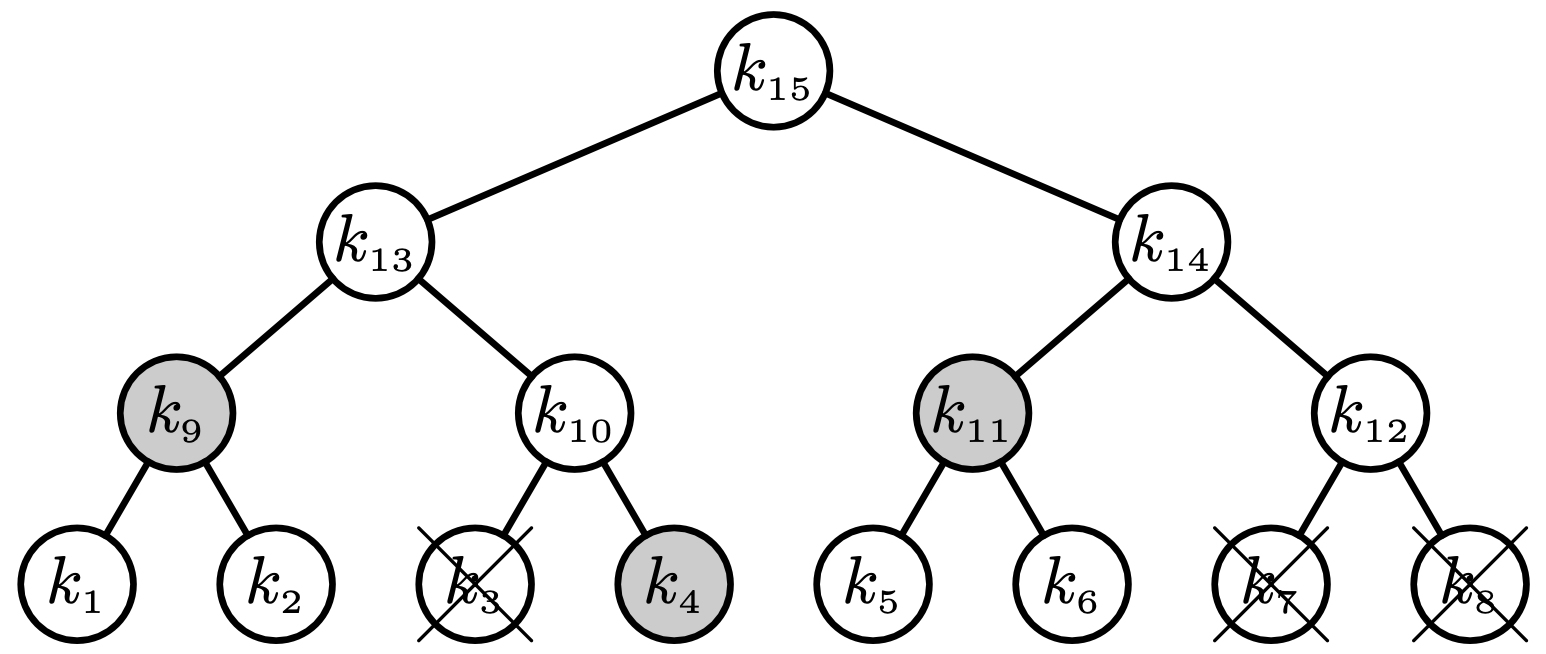
\includegraphics[width=0.45\linewidth]{figures/chapter5/fig6.png}
%  \caption{三个被阴影标记的结点是叶子集 $\{1,2,4,5,6\}$ 的最小覆盖。}
%  \label{fig:5-6}
%\end{figure}

\begin{figure}
  \centering
  

\tikzset{every picture/.style={line width=0.75pt}} %set default line width to 0.75pt        

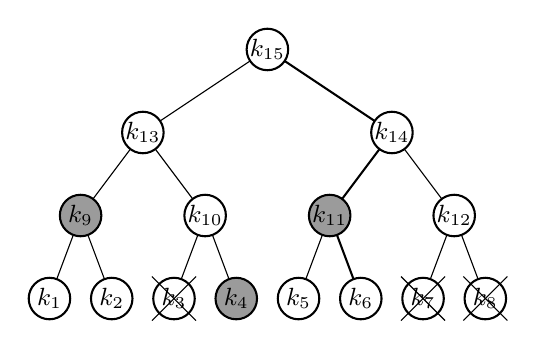
\begin{tikzpicture}[x=0.75pt,y=0.75pt,yscale=-1,xscale=1]
%uncomment if require: \path (0,156); %set diagram left start at 0, and has height of 156

%Straight Lines [id:da7264618821071116] 
\draw    (25,90) -- (10,130) ;
%Straight Lines [id:da021214228424441206] 
\draw    (25,90) -- (40,130) ;
%Straight Lines [id:da7682983898858589] 
\draw    (85,90) -- (70,130) ;
%Straight Lines [id:da680770082896881] 
\draw    (85,90) -- (100,130) ;
%Straight Lines [id:da801506955071976] 
\draw    (145,90) -- (130,130) ;
%Straight Lines [id:da043152738546742064] 
\draw [line width=0.75]    (145,90) -- (160,130) ;
%Straight Lines [id:da8853377273892189] 
\draw    (205,90) -- (190,130) ;
%Straight Lines [id:da7252869978645777] 
\draw    (205,90) -- (220,130) ;
%Straight Lines [id:da02572385855624737] 
\draw    (55,50) -- (25,90) ;
%Straight Lines [id:da30458044388997774] 
\draw    (55,50) -- (85,90) ;
%Straight Lines [id:da17661087510957563] 
\draw [line width=0.75]    (175,50) -- (145,90) ;
%Straight Lines [id:da6362344930800443] 
\draw    (175,50) -- (205,90) ;
%Straight Lines [id:da9010420336797604] 
\draw    (115,10) -- (55,50) ;
%Straight Lines [id:da9254861663329741] 
\draw [line width=0.75]    (115,10) -- (175,50) ;
%Shape: Circle [id:dp5148351832942917] 
\draw  [fill={rgb, 255:red, 255; green, 255; blue, 255 }  ,fill opacity=1 ][line width=0.75]  (0,130) .. controls (0,124.48) and (4.48,120) .. (10,120) .. controls (15.52,120) and (20,124.48) .. (20,130) .. controls (20,135.52) and (15.52,140) .. (10,140) .. controls (4.48,140) and (0,135.52) .. (0,130) -- cycle ;
%Shape: Circle [id:dp8202362949298456] 
\draw  [fill={rgb, 255:red, 255; green, 255; blue, 255 }  ,fill opacity=1 ][line width=0.75]  (30,130) .. controls (30,124.48) and (34.48,120) .. (40,120) .. controls (45.52,120) and (50,124.48) .. (50,130) .. controls (50,135.52) and (45.52,140) .. (40,140) .. controls (34.48,140) and (30,135.52) .. (30,130) -- cycle ;
%Shape: Circle [id:dp29796828256931085] 
\draw  [fill={rgb, 255:red, 255; green, 255; blue, 255 }  ,fill opacity=1 ][line width=0.75]  (60,130) .. controls (60,124.48) and (64.48,120) .. (70,120) .. controls (75.52,120) and (80,124.48) .. (80,130) .. controls (80,135.52) and (75.52,140) .. (70,140) .. controls (64.48,140) and (60,135.52) .. (60,130) -- cycle ;
%Shape: Circle [id:dp27916620429373196] 
\draw  [fill={rgb, 255:red, 155; green, 155; blue, 155 }  ,fill opacity=1 ][line width=0.75]  (90,130) .. controls (90,124.48) and (94.48,120) .. (100,120) .. controls (105.52,120) and (110,124.48) .. (110,130) .. controls (110,135.52) and (105.52,140) .. (100,140) .. controls (94.48,140) and (90,135.52) .. (90,130) -- cycle ;
%Shape: Circle [id:dp29565933370139774] 
\draw  [fill={rgb, 255:red, 255; green, 255; blue, 255 }  ,fill opacity=1 ][line width=0.75]  (120,130) .. controls (120,124.48) and (124.48,120) .. (130,120) .. controls (135.52,120) and (140,124.48) .. (140,130) .. controls (140,135.52) and (135.52,140) .. (130,140) .. controls (124.48,140) and (120,135.52) .. (120,130) -- cycle ;
%Shape: Circle [id:dp025397782343626663] 
\draw  [fill={rgb, 255:red, 255; green, 255; blue, 255 }  ,fill opacity=1 ][line width=0.75]  (150,130) .. controls (150,124.48) and (154.48,120) .. (160,120) .. controls (165.52,120) and (170,124.48) .. (170,130) .. controls (170,135.52) and (165.52,140) .. (160,140) .. controls (154.48,140) and (150,135.52) .. (150,130) -- cycle ;
%Shape: Circle [id:dp653970469885407] 
\draw  [fill={rgb, 255:red, 255; green, 255; blue, 255 }  ,fill opacity=1 ][line width=0.75]  (180,130) .. controls (180,124.48) and (184.48,120) .. (190,120) .. controls (195.52,120) and (200,124.48) .. (200,130) .. controls (200,135.52) and (195.52,140) .. (190,140) .. controls (184.48,140) and (180,135.52) .. (180,130) -- cycle ;
%Shape: Circle [id:dp2542641018476448] 
\draw  [fill={rgb, 255:red, 255; green, 255; blue, 255 }  ,fill opacity=1 ][line width=0.75]  (210,130) .. controls (210,124.48) and (214.48,120) .. (220,120) .. controls (225.52,120) and (230,124.48) .. (230,130) .. controls (230,135.52) and (225.52,140) .. (220,140) .. controls (214.48,140) and (210,135.52) .. (210,130) -- cycle ;
%Shape: Circle [id:dp7410189340861388] 
\draw  [fill={rgb, 255:red, 155; green, 155; blue, 155 }  ,fill opacity=1 ][line width=0.75]  (15,90) .. controls (15,84.48) and (19.48,80) .. (25,80) .. controls (30.52,80) and (35,84.48) .. (35,90) .. controls (35,95.52) and (30.52,100) .. (25,100) .. controls (19.48,100) and (15,95.52) .. (15,90) -- cycle ;
%Shape: Circle [id:dp11686287881251745] 
\draw  [fill={rgb, 255:red, 255; green, 255; blue, 255 }  ,fill opacity=1 ][line width=0.75]  (75,90) .. controls (75,84.48) and (79.48,80) .. (85,80) .. controls (90.52,80) and (95,84.48) .. (95,90) .. controls (95,95.52) and (90.52,100) .. (85,100) .. controls (79.48,100) and (75,95.52) .. (75,90) -- cycle ;
%Shape: Circle [id:dp9012744756772677] 
\draw  [fill={rgb, 255:red, 155; green, 155; blue, 155 }  ,fill opacity=1 ][line width=0.75]  (135,90) .. controls (135,84.48) and (139.48,80) .. (145,80) .. controls (150.52,80) and (155,84.48) .. (155,90) .. controls (155,95.52) and (150.52,100) .. (145,100) .. controls (139.48,100) and (135,95.52) .. (135,90) -- cycle ;
%Shape: Circle [id:dp24117777074385538] 
\draw  [fill={rgb, 255:red, 255; green, 255; blue, 255 }  ,fill opacity=1 ][line width=0.75]  (195,90) .. controls (195,84.48) and (199.48,80) .. (205,80) .. controls (210.52,80) and (215,84.48) .. (215,90) .. controls (215,95.52) and (210.52,100) .. (205,100) .. controls (199.48,100) and (195,95.52) .. (195,90) -- cycle ;
%Shape: Circle [id:dp3084697229561302] 
\draw  [fill={rgb, 255:red, 255; green, 255; blue, 255 }  ,fill opacity=1 ][line width=0.75]  (45,50) .. controls (45,44.48) and (49.48,40) .. (55,40) .. controls (60.52,40) and (65,44.48) .. (65,50) .. controls (65,55.52) and (60.52,60) .. (55,60) .. controls (49.48,60) and (45,55.52) .. (45,50) -- cycle ;
%Shape: Circle [id:dp3751790613196788] 
\draw  [fill={rgb, 255:red, 255; green, 255; blue, 255 }  ,fill opacity=1 ][line width=0.75]  (165,50) .. controls (165,44.48) and (169.48,40) .. (175,40) .. controls (180.52,40) and (185,44.48) .. (185,50) .. controls (185,55.52) and (180.52,60) .. (175,60) .. controls (169.48,60) and (165,55.52) .. (165,50) -- cycle ;
%Shape: Circle [id:dp9802416358387074] 
\draw  [fill={rgb, 255:red, 255; green, 255; blue, 255 }  ,fill opacity=1 ][line width=0.75]  (105,10) .. controls (105,4.48) and (109.48,0) .. (115,0) .. controls (120.52,0) and (125,4.48) .. (125,10) .. controls (125,15.52) and (120.52,20) .. (115,20) .. controls (109.48,20) and (105,15.52) .. (105,10) -- cycle ;
\draw   (59.39,119.39) -- (80.61,140.61)(80.61,119.39) -- (59.39,140.61) ;
\draw   (179.39,119.39) -- (200.61,140.61)(200.61,119.39) -- (179.39,140.61) ;
\draw   (209.39,119.39) -- (230.61,140.61)(230.61,119.39) -- (209.39,140.61) ;

% Text Node
\draw (115,10) node  [font=\small]  {$k_{15}$};
% Text Node
\draw (55,50) node  [font=\small]  {$k_{13}$};
% Text Node
\draw (85,90) node  [font=\small]  {$k_{10}$};
% Text Node
\draw (70,130) node  [font=\small]  {$k_{3}$};
% Text Node
\draw (25,90) node  [font=\small]  {$k_{9}$};
% Text Node
\draw (10,130) node  [font=\small]  {$k_{1}$};
% Text Node
\draw (40,130) node  [font=\small]  {$k_{2}$};
% Text Node
\draw (100,130) node  [font=\small]  {$k_{4}$};
% Text Node
\draw (130,130) node  [font=\small]  {$k_{5}$};
% Text Node
\draw (160,130) node  [font=\small]  {$k_{6}$};
% Text Node
\draw (190,130) node  [font=\small]  {$k_{7}$};
% Text Node
\draw (220,130) node  [font=\small]  {$k_{8}$};
% Text Node
\draw (145,90) node  [font=\small]  {$k_{11}$};
% Text Node
\draw (205,90) node  [font=\small]  {$k_{12}$};
% Text Node
\draw (175,50) node  [font=\small]  {$k_{14}$};


\end{tikzpicture}
  \caption{三个被阴影标记的结点是叶子集 $\{1,2,4,5,6\}$ 的最小覆盖。}
  \label{fig:5-6}
\end{figure}

被撤销的设备越多,$c_\mathrm{m}$ 的密文头部就越大。下面的定理显示了在最坏的情况下密文头部会有多大。该证明是一个归纳论证,它还给出了一种用于计算最优覆盖的高效递归算法。

\begin{theorem}\label{theo:5-8}
令 $T$ 是一棵包含 $n$ 个叶子结点的完全二叉树,其中 $n$ 是$2$ 的整数次幂。对于每个 $1\leq r\leq n$ 以及每个包含 $n-r$ 个叶子结点的集合 $S$,我们都有:
\[
|\mathrm{cover}(S)|\leq r\cdot\log_2(n/r)
\]
\end{theorem}

\begin{proof}
我们通过在 $\log_2n$ 上的归纳法来证明该定理,当 $n=1$ 时,该定理显然成立。现在,假设该定理在有 $n/2$ 个叶子结点的树上成立,我们想要证明该定理在有 $n$ 个叶子结点的树 $T$ 上仍然成立。树 $T$ 由一个根结点和两颗不相交的子树 $T_1$ 和 $T_2$ 组成,而每颗子树都有 $n/2$ 个叶子结点。让我们把集合 $S\subseteq\{1,\dots,n\}$ 一分为二,即 $S=S_1\cup S_2$,其中 $S_1$ 包含在集合 $\{1,\dots,n/2\}$ 中,$S_2$ 包含在集合 $\{n/2+1,\dots,n\}$ 中。也就是说,$S_1$ 是 $S$ 中属于 $T_1$ 的元素,$S_2$ 是 $S$ 中属于 $T_2$ 的元素。令 $r_1:=(n/2)-|S_1|$,$r_2:=(n/2)-|S_2|$。那么,显然有 $r=r_1+r_2$。

首先,假设 $r_1$ 和$r_2$ 都大于零。根据归纳假设,我们知道对于 $i=1,2$,我们有 $|\mathrm{cover}(S_i)|\leq r_i\log_2(n/2r_i)$ 成立。因此:
\[
\begin{aligned}
|\mathrm{cover}(S)| & = |\mathrm{cover}(S_1)| + |\mathrm{cover}(S_2)| \leq r_1\log_2(n/2r_1)+r_2\log_2(n/2r_2)\\
& = r\log_2(n/r) + \big(r\log_2r-r_1\log_2(2r_1)-r_2\log_2(2r_2)\big) \leq r\log_2(n/r)
\end{aligned}
\]
这就是我们在归纳中想要证明的。最后一个不等式来自于一个关于对数的简单事实,即对于所有的 $r_1\geq1$ 和 $r_2\geq1$,我们都有:
\[
(r_1+r_2)\log_2(r_1+r_2)\leq r_1\log_2(2r_1)+r_2\log_2(2r_2)
\]

其次,如果 $r_1=0$,那么 $r_2=r\geq1$。现在,归纳可以由以下论证得出:
\[
|\mathrm{cover}(S)| = |\mathrm{cover}(S_2)| \leq r\log_2(n/2r) = r\log_2(n/r)-r \leq r\log_2(n/r)
\]
这符合要求。$r_2=0$ 的情况与此类似,不再赘述。这就完成了归纳,进而完成了对本定理的证明。
\end{proof}

定理 \ref{theo:5-8} 表明,撤销 $r$ 台设备的代价是将密文头部的大小增加到 $r\log_2(n/r)$ 个分组。对于大小适当的 $r$,这个值并不是太大。尽管如此,这种普适的方法仍然可以被改进。使用该方法的最佳系统在每个设备中嵌入 $O(\log n)$ 个密钥,与这里相同,但密文头部的大小只有 $O(r)$ 个分组。AACS 系统使用了子集树差异法,在最坏的情况下,密文头部的大小为 $2r-1$ 个分组,但每个设备只需存储 $1/2\log_2n$ 个密钥。

虽然 AACS 的设计远比 CSS 好,但它也同样被攻破了。特别是,撤销 AACS 密钥的过程是相当复杂的,可能需要好几个月。黑客的攻击表明,他们可以从未撤销的播放器中提取新的设备密钥,其速度比业界撤销密钥的速度还要快。